\documentclass[a4paper,12pt]{article}
\usepackage[utf8x]{inputenc} %fac
%\usepackage[utf8]{inputenc} %fac

%\usepackage[square,sort,comma]{natbib}
%\usepackage{chapterbib}

\usepackage[english]{babel} %FR
\usepackage[T1]{fontenc}
\usepackage{fancyhdr}
\usepackage{caption} %multiline caption

\usepackage[pdftex]{graphicx} % img
%\usepackage{wrapfig} %fac
\usepackage{float}

%\usepackage{algpseudocode} %fac/


\usepackage[top=3cm, bottom=3cm, left=2.5cm, right=2.5cm]{geometry} %Réduire les marges

% \usepackage{showkeys}
% \usepackage{showlabels}
\usepackage{nameref}

\usepackage{amsmath}


% Style Page
\pagestyle{fancy} % entêtes

\setlength{\headheight}{15pt}
\lhead{ \leftmark }
\rhead{ %\rightmark 
}



\sloppy % ne pas faire déborder les lignes dans la marge

\usepackage[hidelinks]{hyperref} %fac

%\setcounter{tocdepth}{1} %hideallsubsections

%\setcounter{secnumdepth}{5}
%\setcounter{tocdepth}{5}

\graphicspath{{images/}}

\begin{document}
  \begin{titlepage}
  \def\titletype{Experiments}
   \def\majortitle{Learning from expert}
   \def\docversion{1.0}
   %%%%%%%%%%%%%%%%%%%%%%%%%%%%%%%%%%%%%%%%%
% University Assignment Title Page
% LaTeX Template
%
% This template has been downloaded from:
% http://www.latextemplates.com
%
% Original author:
% WikiBooks (http://en.wikibooks.org/wiki/LaTeX/Title_Creation)
%
% Instructions for using this template:
% This title page is presently capable of being compiled as is. This is not
% useful for including it in another document. To do this, you have two options:
%
% 1) Copy/paste everything between \begin{document} and \end{document}
% starting at \begin{titlepage} and paste this into another LaTeX file where you
% want your title page.
% OR
% 2) Remove everything outside the \begin{titlepage} and \end{titlepage} and
% move this file to the same directory as the LaTeX file you wish to add it to.
% Then add \input{./title_page_1.tex} to your LaTeX file where you want your
% title page.
%
%%%%%%%%%%%%%%%%%%%%%%%%%%%%%%%%%%%%%%%%%

%----------------------------------------------------------------------------------------
%       PACKAGES AND OTHER DOCUMENT CONFIGURATIONS
%----------------------------------------------------------------------------------------

\begin{titlepage}

\newcommand{\HRule}{\rule{\linewidth}{0.5mm}} % Defines a new command for the horizontal lines, change thickness here

\center % Center everything on the page

%----------------------------------------------------------------------------------------
%       HEADING SECTIONS
%----------------------------------------------------------------------------------------

\textsc{\LARGE Pierre and Marie Curie University}\\[1.5cm] % Name of your university/college
\textsc{\Large \titletype}\\[0.5cm] % Major heading such as course name
%\textsc{\large PIAD de Master1 d’Informatique en Intelligence Artificielle et Décision}\\[0.5cm] % Minor heading such as course title

%----------------------------------------------------------------------------------------
%       TITLE SECTION
%----------------------------------------------------------------------------------------

\HRule \\[0.4cm]
{ \huge \bfseries \majortitle}\\[0.4cm] % Title of your document
\HRule \\[1.5cm]


%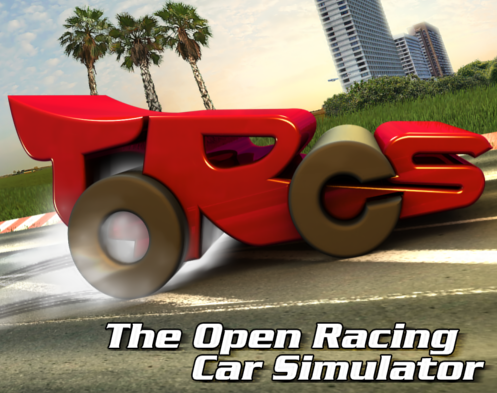
\includegraphics[height=60mm]{images/torcs.png}\\[1cm]


%----------------------------------------------------------------------------------------
%       AUTHOR SECTION
%----------------------------------------------------------------------------------------

\begin{minipage}{0.4\textwidth}
\begin{flushleft} \large
\emph{Author:}\\
Matthieu \textsc{Zimmer} % Your name
\end{flushleft}
\end{minipage}
~
\begin{minipage}{0.4\textwidth}
\begin{flushright} \large
\emph{Supervisors:} \\
Paolo \textsc{Viappiani}\\ % Supervisor's Name
Paul \textsc{Weng}\\ % Supervisor's Name
\end{flushright}
\end{minipage}\\[1cm]

\vfill

%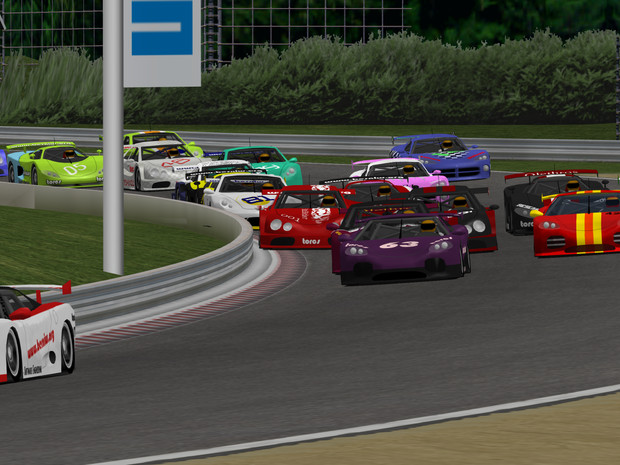
\includegraphics[height=70mm]{images/torcs.jpg}\\[1cm]

%----------------------------------------------------------------------------------------
%       DATE SECTION
%----------------------------------------------------------------------------------------

{\large \today}\\[3mm] % Date, change the \today to a set date if you want to be precise
{\large Version \docversion}\\[1.5cm]

%----------------------------------------------------------------------------------------
%       LOGO SECTION
%----------------------------------------------------------------------------------------


\includegraphics[height=13mm]{../images/logo.png} % Include a department/university logo - this will require the graphicx package

%----------------------------------------------------------------------------------------

% \vfill % Fill the rest of the page with whitespace

\end{titlepage}

  \end{titlepage}

  
  \clearpage

  \tableofcontents
%   \addcontentsline{toc}{section}{Table de matière}
  
  %\vfill
  %\begin{center}
  %  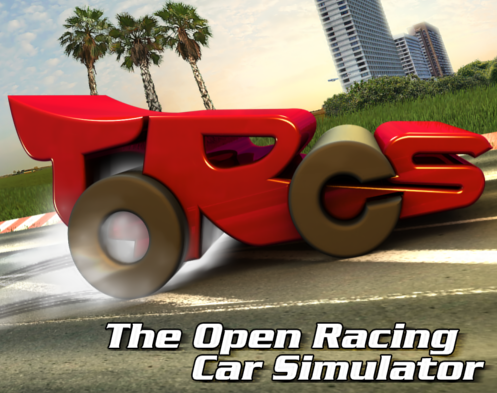
\includegraphics[height=90mm]{images/torcs.png} 
  %\end{center}

  \clearpage
  
  \renewcommand{\labelitemi}{$\bullet$}
  \renewcommand{\labelitemii}{$\circ$}
  \renewcommand{\labelitemiii}{$\diamond$}
  \renewcommand{\labelitemiv}{$\ast$}
  
%   \section{Cadre : Apprentissage non supervisé par apprentissage des densités}

  \clearpage
  \section{Environnement}
    \subsection{Mountain car}

    A standard testing domain in reinforcement learning, is a problem in which an under-powered 
    car must drive up a steep hill. Since gravity is stronger than the car's engine, even at full 
    throttle, the car cannot simply accelerate up the steep slope. The car is situated in a valley
    and must learn to leverage potential energy by driving up the opposite hill before the car is 
    able to make it to the goal at the top of the rightmost hill.
    \begin{figure}[H]
      \begin{center}
	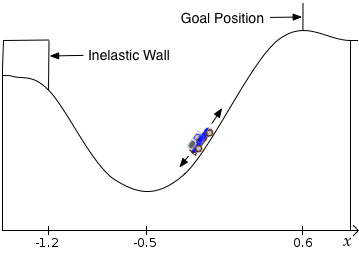
\includegraphics[width=270px]{Mcar}
	\caption{ The Mountain Car Problem }
	\end{center}
    \end{figure}
    
    \subsubsection{State Variables}
    Two dimensional continuous state space : Velocity = (-0.07,0.07) and Position = (-1.2,0.6)
    
    \subsubsection{Actions}
     One dimensional discrete action space : Motor = (left, neutral, right)
     
     \subsubsection{Reward}
      For every time step: -1, when goal is reached: +1

    \subsubsection{Update Function}
    Velocity = Velocity + Action *0.001+cos(3*Position)*-0.0025
    \newline Position = Position + Velocity

    \subsubsection{Starting Condition}
    Position = -0.5 Velocity = 0.0
    
    \subsubsection{Termination Condition}
    Position >= 0.6
    
    
    
    \subsection{Grid Game}

The mountain car problem gives a -1 reward at every step, and the state allows to 
    determine exactly the best action to take. So we could think that there is no state more important than other (to give feedbacks). 

Here, we introduce an other problem where rewards will be different according to our state.
    
    The agent have to reach every green boxes in the given order.

    \begin{figure}[H]
      \begin{center}
	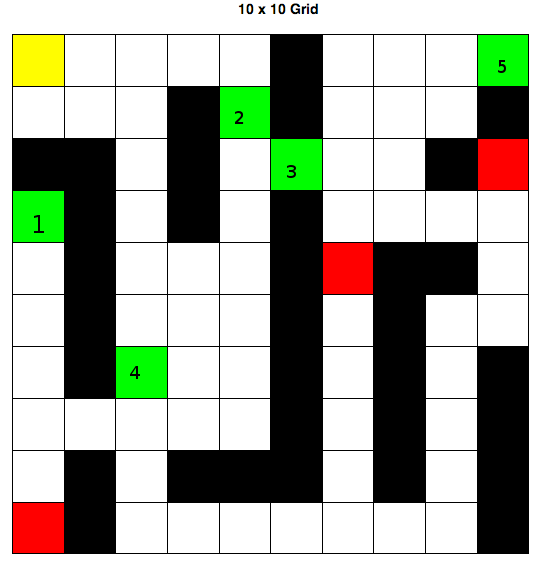
\includegraphics[width=270px]{gridworld}
	\caption{ Grid World }
	\end{center}
    \end{figure}
    
    \subsubsection{State Variables}
    Four dimensional discretized state space :\newline
    X = \{0, 9\} ; Y = \{0, 9\} ; XGOAL = \{0, 9\} ; YGOAL = \{0, 9\}
    
    \subsubsection{Actions}
    One dimensional discrete action space : Direction = (left, up, right, bottom)

     \subsubsection{Reward}
      white boxes : -1 \newline
      green boxes : +10 (only the first time)\newline
      red boxes : -10 \newline
    
    \subsection{Second Grid Game (LS)}

    The main difference in this problem, is that, given a state there isn't only one best possible action.
     
    The agent have to reach every green boxes in any order.

    \begin{figure}[H]
      \begin{center}
	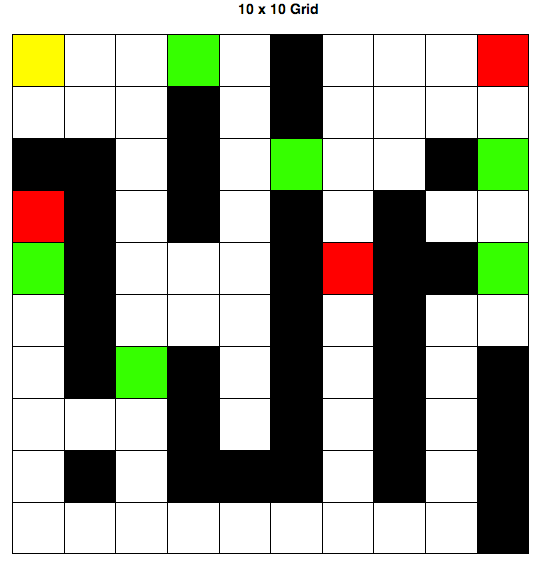
\includegraphics[width=270px]{gridworldls}
	\caption{ Gris World Insconsistent State }
	\end{center}
    \end{figure}
    
    \subsubsection{State Variables}
    Four dimensional discretized state space : X = \{0, 9\} ; Y = \{0, 9\}
    
    \subsubsection{Actions}
     One dimensional discrete action space : Direction = (left, up, right, bottom)
     
     \subsubsection{Reward}
      white boxes : -1 \newline
      green boxes : +10 (only the first time)\newline
      red boxes : -10 \newline
      
      \subsubsection{State inconsistency}
      
      Imagine your in the boxe (6,0), you only know that you are in this box, you don't already know 
      if you reach the goal in (4,0). Thus, there is two different reasonable chooses.

      \section{Comparing strategy : how the advice affects the learner}
      \subsection{Strategies}
      \subsubsection{Max}
       $Q(s,a) = max(Q(s,\_)) + \delta$
       \subsubsection{Override (Lucky Exploration)}
       $\pi(s)=a$ \newline
       $Q(s,a)$ will be updating according with the reward given the next time in this state.
       \subsubsection{Max + Override}
	$\pi(s)=a$ \newline
	$Q(s,a) = max(Q(s,\_) + \delta$

	\subsubsection{Others}
      We could imagine an other strategy as Lucky Exploration only for 
      the next time we encounter this state ( not fixed for everytime ).
      
      \subsection{Experiment A : Advice after}
      In this experiment, we have two agent, a teacher (QLearning) and a learner (QLearning).
      The teacher is favored to advice (it is done to compare advice effects) : +10 if advice
      else -10. With this reward function, it is not important to display the algorithm ``advice before''
      because it will advice all the time.
      
      The teacher advices the learner with the best action to take (according to 
      the best policy previously computed). They have the same state representation.
            
      \subsubsection{Mountain Car}
      \begin{figure}[H]
      \begin{center}
	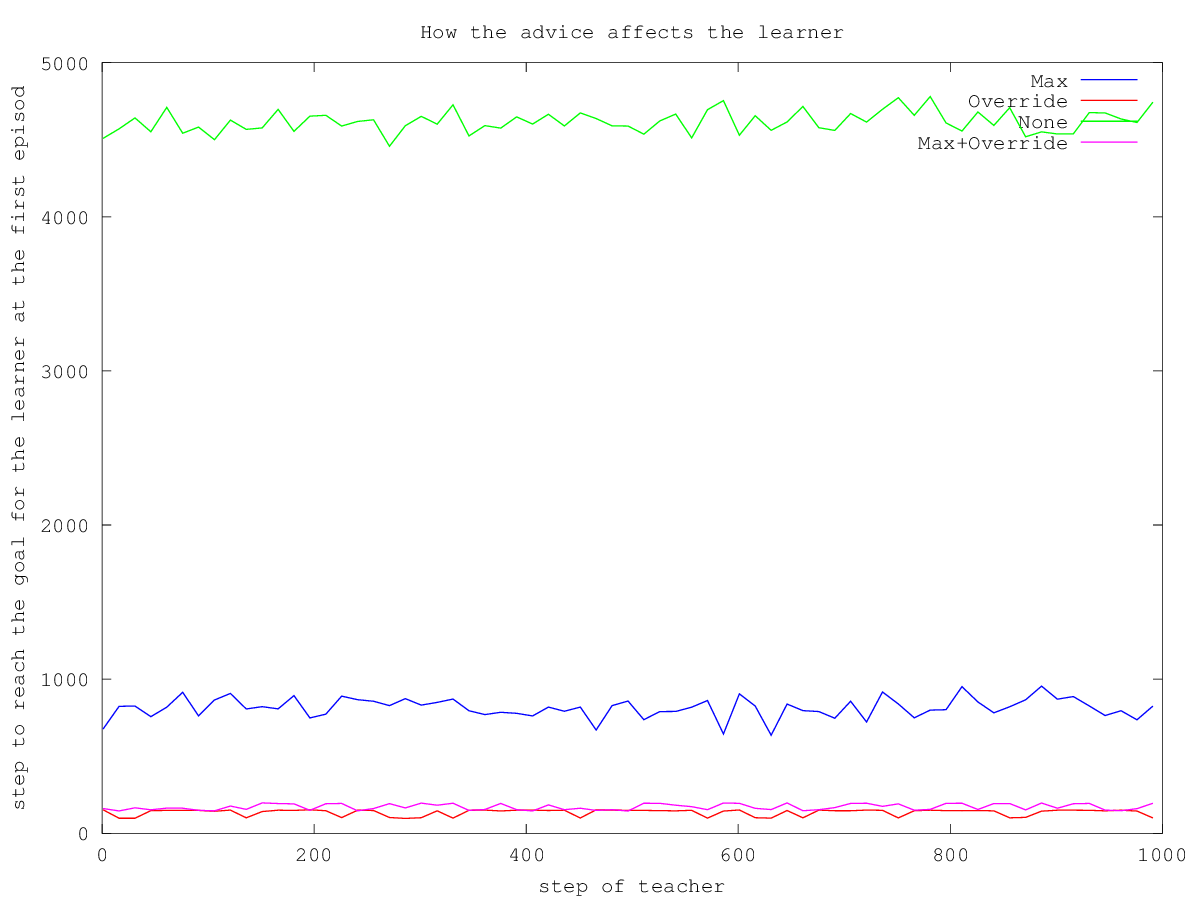
\includegraphics[width=320px]{graphA_MA}
	\caption{ Teacher advices all the time. Number of step to reach to goal at the first episod }
	\end{center}
      \end{figure}
      
      The two best strategies are Override and Max+Override. (Max+Override is a little quite better because it
      updates the Q value directly).
%       Moreover, the Max strat is really better but 
      
      \subsubsection{Grid World}
      \begin{figure}[H]
      \begin{center}
	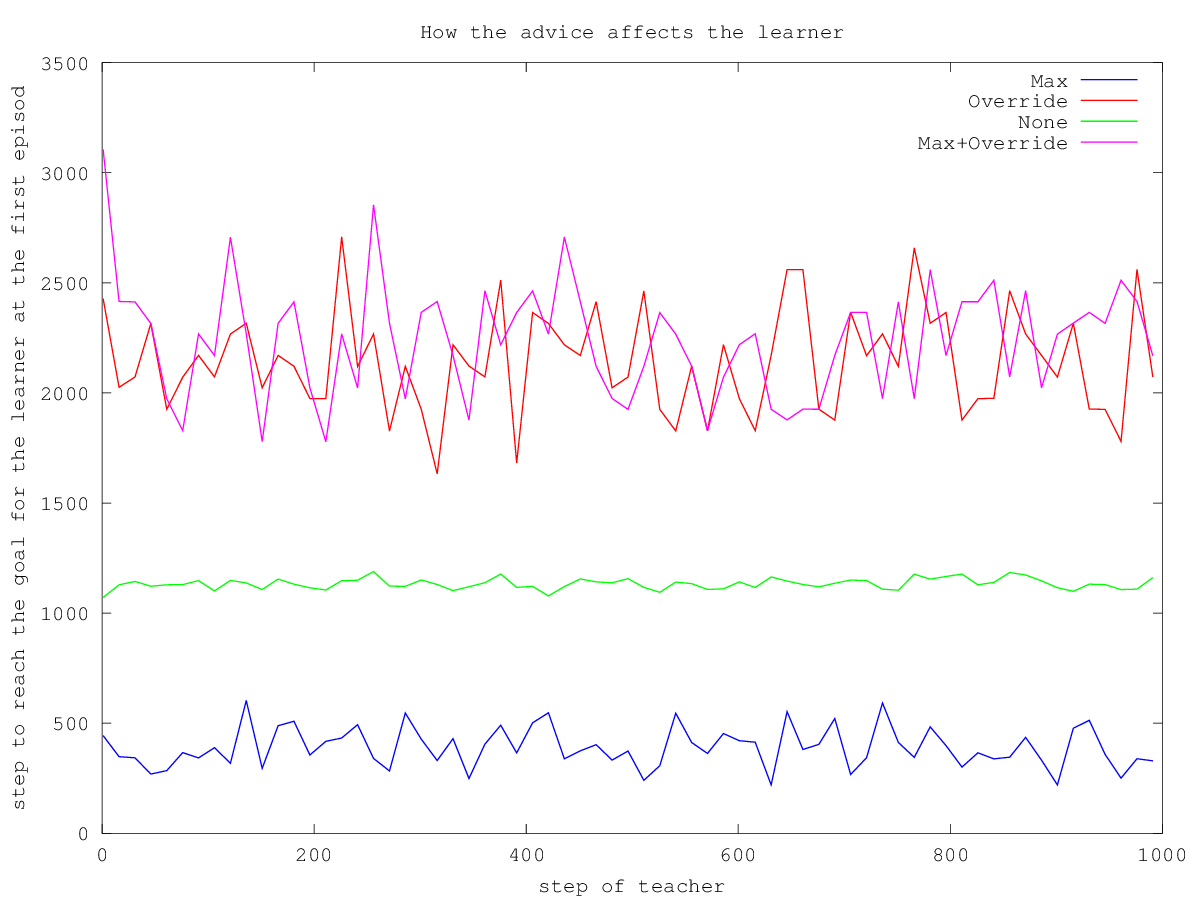
\includegraphics[width=320px]{graphA_GA}
	\caption{ Teacher advices all the time. Number of step to reach to goal at the first episod }
	\end{center}
      \end{figure}
      
      This time in the grid world, the best strategy is Max.
      The fixed policy strat are really bad, more than without advice.
      
      \subsubsection{Grid World (LS)}
      \begin{figure}[H]
      \begin{center}
	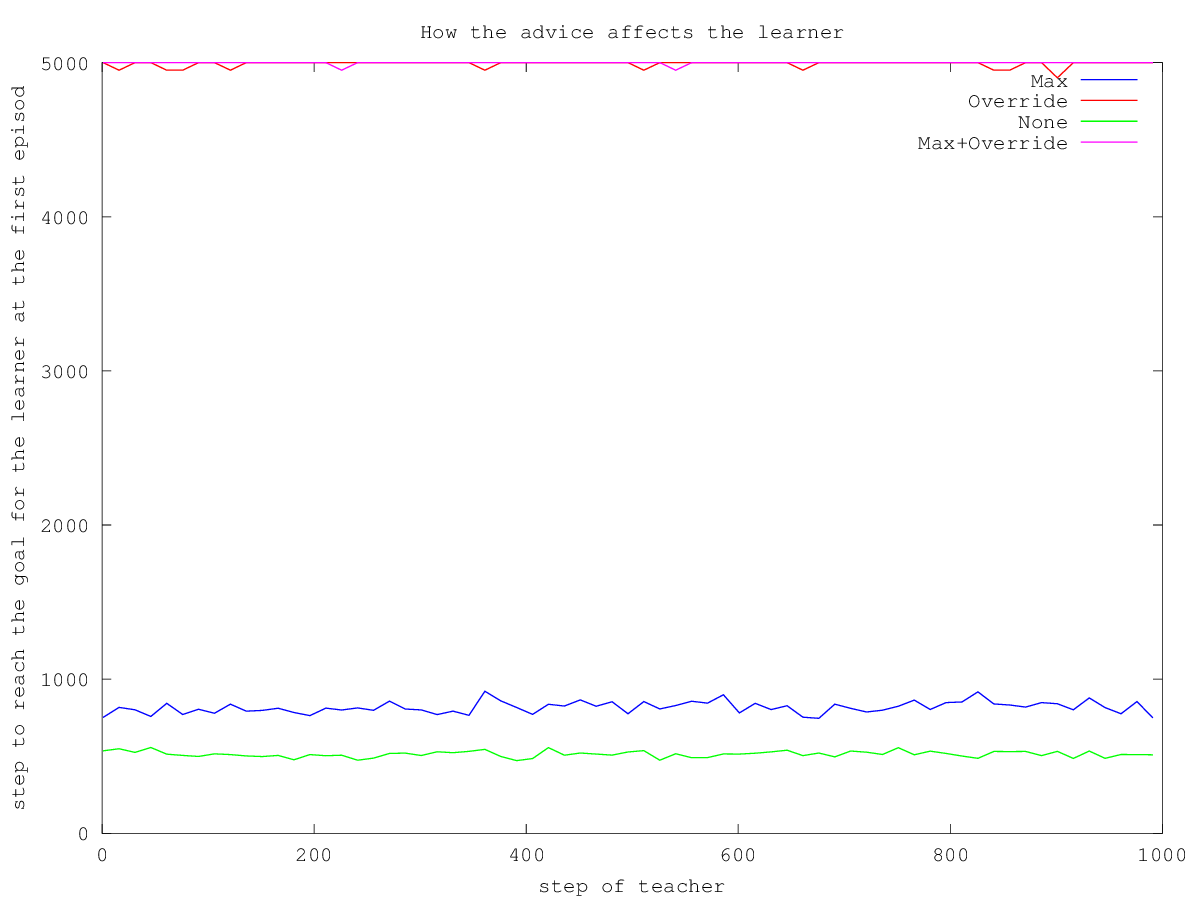
\includegraphics[width=320px]{graphA_LA}
	\caption{ Teacher advices all the time. Number of step to reach to goal at the first episod }
	\end{center}
      \end{figure}
      
      In this environnement, all strategies are bad when the teacher advice after because of 
      the different good choose possible in a same state.
      
      
      \subsection{Experiment B : Advice before}
      
      This experiment is used to compare the advice effect when the teacher can correct a mistake of the 
      learner before he perform it.
      Also, we need to use a different reward function (based on a cost when he advice) for the teacher, 
      otherwise he will advice always and all algorithms will be at the same performance.
      
      \section{Comparing teaching strategies : teacher reward function}
      
      \subsection{Reward functions}
%       \begin{itemize}
%        \item Max
%        
%        \item Max + Override
%        \item Override (Lucky Exploration)
%       \end{itemize}



    %     \begin{center}
%       ${CM}^* = \underset{CM}{\operatorname{argmax}}\ p( S_1,...,S_n | CM ) $
%     \end{center}
%     \begin{center}
%       $p( S_1,...,S_n | CM ) = p(S_1|CM) \times \prod\limits_{i=2}^n p(S_i|S_{i-1}, CM)$
%     \end{center}
%     
%     Par ailleurs, nous allons nous concentrer sur les arrondissements du
%     $4^{i\grave{e}me}$ et du $16^{i\grave{e}me}$ arrondissement.
% 
%     \subsubsection{Données bruts}
% 
%       Moyennes réalisées sur une centaine de lancement.
%       
%       \begin{center}
% 	\begin{tabular}{cc}
% 	  \hspace*{-1cm}
% 	  \begin{minipage}[b]{.52\linewidth}
% 	    \begin{figure}[H]
% % 	      \includegraphics[width=270px]{e32call}
% 	      \caption{ Taux de classification  }
% 	    \end{figure}
% 	  \end{minipage}
% 	  &
% 	  \begin{minipage}[b]{.5\linewidth}
% 	    \begin{figure}[H]
% % 	      \includegraphics[width=270px]{e32calln}
% 	      \caption{ Taux avec normalisation  }
% 	    \end{figure}
% 	  \end{minipage}
% 	\end{tabular}
%       \end{center} 
%       
%       La première chose que l'on peut remarquer est l'interêt de la discrétisation des données puisque sans elle
%       on ne peut dépasser les 25\% de performance. Néanmoins, il ne faut pas créer de classe trop grande puisque
%       qu'au delà des intervales de taille 10, les performances vont diminuer petit à petit.
%       
%       La seconde information est celle de l'interêt de la normalisation, qui, comme on peut le voir ici, n'influe que
%       très peu sur les résultats.
%     
%     \subsubsection{Données différentielles}
%     
%     Nous allons maintenant utiliser un autre codage des données et modéliser le nombre de vélib arrivant ou partant
%     pour une station donnée. Ce sont également des moyennes réalisées sur une centaine de lancement.
%     
% 	\begin{center}
% 	\begin{tabular}{cc}
% 	  \hspace*{-1cm}
% 	  \begin{minipage}[b]{.52\linewidth}
% 	    \begin{figure}[H]
% % 	      \includegraphics[width=270px]{e32calls}
% 	      \caption{ Taux de classification  }
% 	    \end{figure}
% 	  \end{minipage}
% 	  &
% 	  \begin{minipage}[b]{.5\linewidth}
% 	    \begin{figure}[H]
% % 	      \includegraphics[width=270px]{e32callsn}
% 	      \caption{ Taux avec normalisation  }
% 	    \end{figure}
% 	  \end{minipage}
% 	\end{tabular}
%       \end{center} 
%     
%     
%     \subsection{Clustering}
%     
%     Nous allons maintenant utiliser les chaînes de Markov pour faire du clustering. Nous nous plaçons donc dans
%     le cadre de l'apprentissage non supervisé. Pour réaliser le clustering, nous utiliserons la famille d'algorithme
%     EM. Nous aurons une chaine de Markov par cluster que nous optimiserons.
%     
%     
%     \subsubsection{Données}
%     
%     Nous allons utiliser les mêmes données que précédent mais en prenant en compte tout les arrondissements de Paris.
%     
%     \begin{figure}[H]
%       \begin{center}
% % 	\includegraphics[width=270px]{paris}
% 	\caption{ Stations dans Paris }
% 	\end{center}
%     \end{figure}
%       
%     
%     \subsection{Clustering en pré-traitement}
%     
%     Il peut être interessant de prétraiter la classification par un clustering pour réduire la dimensionnalité des données
%     avant de les traiter.
%   
%   \section{Modèles de Markov Cachés}

      
      


      
%       \begin{figure}[H]
%       \begin{center}
% 	\includegraphics[width=270px]{donnes_gaussians}
% 	\caption{ Données gaussiennes linéairement séparables.\newline La frontrière est déterminer par adaline. }
% 	\end{center}
%       \end{figure}
%       
%       

%       	\begin{center}
% 	\begin{tabular}{cc}
% 	  \hspace*{-1cm}
% 	  \begin{minipage}[b]{.5\linewidth}
% 	    \begin{figure}[H]
% 	      \includegraphics[width=265px]{grad_convR}
% 	      \caption{ Evolution du critère d'erreur\\ en fonction des itérations. }
% 	    \end{figure}
% 	  \end{minipage}
% 	  &
% 	  \begin{minipage}[b]{.5\linewidth}
% 	    \begin{figure}[H]
% 	      \includegraphics[width=270px]{espaceWR}
% 	      \caption{ Espace du vecteur W\\[0.5cm]}
% 	    \end{figure}
% 	  \end{minipage}
% 	\end{tabular}
%       \end{center} 
      
      
%       
%       \begin{center}
% 	\begin{tabular}{cc}
% 	  \hspace*{-1cm}
% 	  \begin{minipage}[b]{.5\linewidth}
% 	    \begin{figure}[H]
% 	      \includegraphics[width=270px]{grad_convL}
% 	      \caption{ Evolution du critère d'erreur\\ en fonction des itérations. }
% 	    \end{figure}
% 	  \end{minipage}
% 	  &
% 	  \begin{minipage}[b]{.5\linewidth}
% 	    \begin{figure}[H]
% 	      \includegraphics[width=270px]{espaceWL}
% 	      \caption{ Espace du vecteur W\\[0.5cm]}
% 	    \end{figure}
% 	  \end{minipage}
% 	\end{tabular}
%       \end{center} 
      

%       \begin{center}
% 	\begin{tabular}{cc}
% 	  \hspace*{-1cm}
% 	  \begin{minipage}[b]{.5\linewidth}
% 	    \begin{figure}[H]
% 	      \includegraphics[width=270px]{grad_convD}
% 	      \caption{ Evolution du critère d'erreur\\ en fonction des itérations. }
% 	    \end{figure}
% 	  \end{minipage}
% 	  &
% 	  \begin{minipage}[b]{.5\linewidth}
% 	    \begin{figure}[H]
% 	      \includegraphics[width=270px]{espaceWD}
% 	      \caption{ Espace du vecteur W\\[0.5cm]}
% 	    \end{figure}
% 	  \end{minipage}
% 	\end{tabular}
%       \end{center} 
      

  \clearpage
  
%   \clearpage
%   \section{Performances}
%     \subsection{Rejet - knn}
%       \subsubsection{En ambiguité}
%       \subsubsection{En distance}
%     \subsection{Surapprentissage - adaline}
%     \subsection{Surapprentissage - knn}
%     Le surapprentissage de knn peut être visible sur la figure 10.
%     \subsection{Validation croisée - perceptron}
%     \subsection{Validation croisée - knn}

\end{document}



